\documentclass[a4paper,12pt]{article} 

%Добавляет возможность искать и копировать текст
\usepackage{cmap}

%Убирает пробел между названием таблицы/рисунка и самой таблицей/рисунком
\usepackage{caption}
\captionsetup[table]{skip= -0 cm}
\captionsetup[figure]{skip= -0 cm}

%Выравнивание названия таблиц по левому краю
%\usepackage[nooneline]{caption} 
%Размеры отступов 
\usepackage[left=20mm, top=20mm, right=20mm, bottom=20mm, footskip=10mm]{geometry}

%Рисунки
\usepackage{graphicx}
\usepackage{wrapfig} %обтекание элементов
\graphicspath{{graphs}{figures}}  % папки с картинками

%Русский язык в формулах
\usepackage{mathtext}

%  Русский язык
\usepackage[T2A]{fontenc}			
\usepackage[utf8]{inputenc}			
\usepackage[english,russian]{babel}	

%Готические буквы
\usepackage{amssymb}

% Математика
\usepackage{amsmath,amsfonts,amssymb,amsthm,mathtools} 
\usepackage{wasysym}

%Цветные подписи в таблице
\usepackage[table,xcdraw]{xcolor}

\usepackage{fancyhdr} % Колонтитулы
 	\pagestyle{fancy}
 	\renewcommand{\headrulewidth}{0.3mm}  % Толщина линейки, отчеркивающей верхний колонтитул
 	%\lfoot{Нижний левый}
 	%\rfoot{Нижний правый}
 	\rhead{Б04-006}
 	%\chead{Верхний в центре}
 	\lhead{Лабораторная работа №4.3.1}
 	% \cfoot{Нижний в центре} % По умолчанию здесь номер страницы
 	
 	
\begin{document} 

%Титульник 
\begin{titlepage}
	\begin{center}
		\large 	МИНИСТЕРСТВО ОБРАЗОВАНИЯ И НАУКИ РОССИЙСКОЙ ФЕДЕРАЦИИ\\
				МОСКОВСКИЙ ФИЗИКО-ТЕХНИЧЕСКИЙ ИНСТИТУТ \\
				(НАЦИОНАЛЬНЫЙ ИССЛЕДОВАТЕЛЬСКИЙ ИНСТИТУТ)\\ 
				ФИЗТЕХ-ШКОЛА ЭЛЕКТРОНИКИ, ФОТОНИКИ \\
				И МОЛЕКУЛЯРНОЙ ФИЗИКИ \\
		
		
		\vspace{4.0 cm}
		Лабораторная работа № 4.3.1 \\ 
		\LARGE \textbf{Изучение дифракции света}
	\end{center}
	\vspace{3 cm} \large
	
	\begin{flushright}
		выполнили студенты 2 курса \\
		{группы Б04-006}\\
		\textbf{Белостоцкий Артемий}\\
		\textbf{Вовк Дмитрий}\\
	\end{flushright}
	
	\vfill

	\begin{center}
	Долгопрудный, 2022 г.
	\end{center}
\end{titlepage}                                                                      

\section*{Цель работы}

Исследовать явления дифрауции Френеля и Фраунгофера на щели, изучить влияние дифракции на разрешающую способность оптических инструментов.

\section*{В работе используются}

\begin{itemize}
\item оптическая скамья
\item ртутная лампа
\item монохроматор
\item щели с регулируемой шириной 
\item рамка с вертикальной нитью
\item двойная щель
\item микроскоп с микрометрическим винтом на поперечных салазках
\item зрительная труба
\end{itemize}

\section*{Дифракция Френеля}

Соберем схему согласно рис. 1. 

\begin{figure}[h!]
	\begin{center}
    		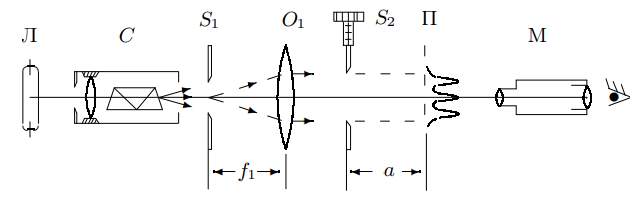
\includegraphics[scale = 1]{fig1}
    		\caption{Схема установки для наблюдения дифракции Френеля}
	\end{center}
\end{figure}

Добившись наибольшей четкости дифракционной картины, найдем резкое изображение щели. Постепенно отодвигая микроскоп от щели $S_2$, отметим положение микроскопа, при котором на фоне щели видна одна темная полоса.

.Приближая микроскоп к щели снимем зависимость координаты микроскопа от числа n наблюдаемых полос. Рассчитаем расстояние -- $a = |z_n - z_0|$ -- смещение микроскопа от положения где n = 0($z_0 = 49,8 см $).Также рассчитаем суммарную ширину n зон Френеля по формуле $z_m = \sqrt{a m \lambda}$ ($\lambda$ = 5480 \AA) . Результаты занесем в Таблицу 1.

\newpage

\begin{table}[h]
\begin{center}
\caption{Зависимость координаты микроскопа от числа n наблюдаемых полос}
\begin{tabular}{|c|c|c|c|c|}
\hline
z, см & n & a, см & $2z_n * 10^3$, см & $\sigma_{2z_n} * 10^3$, см \\ \hline
51,6  & 1 & 0     & 19,82 & 0,78 \\ \hline
50,9  & 2 & 0,7   & 21,92 & 1,41\\ \hline
50,6  & 3 & 1     & 22,90 & 2,02\\ \hline
50,4  & 4 & 1,2   & 22,90 & 2,70\\ \hline
\end{tabular}
\end{center}
\end{table}

где погрешность рассчитывалась по формуле:

$$
\sigma_{2z_m} = 2 \sqrt{\frac{2\lambda n}{a}} \sigma_z,
$$

где $\sigma_z = 0,05 см$

Построим график зависимости $2z_n = f(n)$ и отметим на нем ширину щели.

\begin{figure}[h!]
	\begin{center}
    		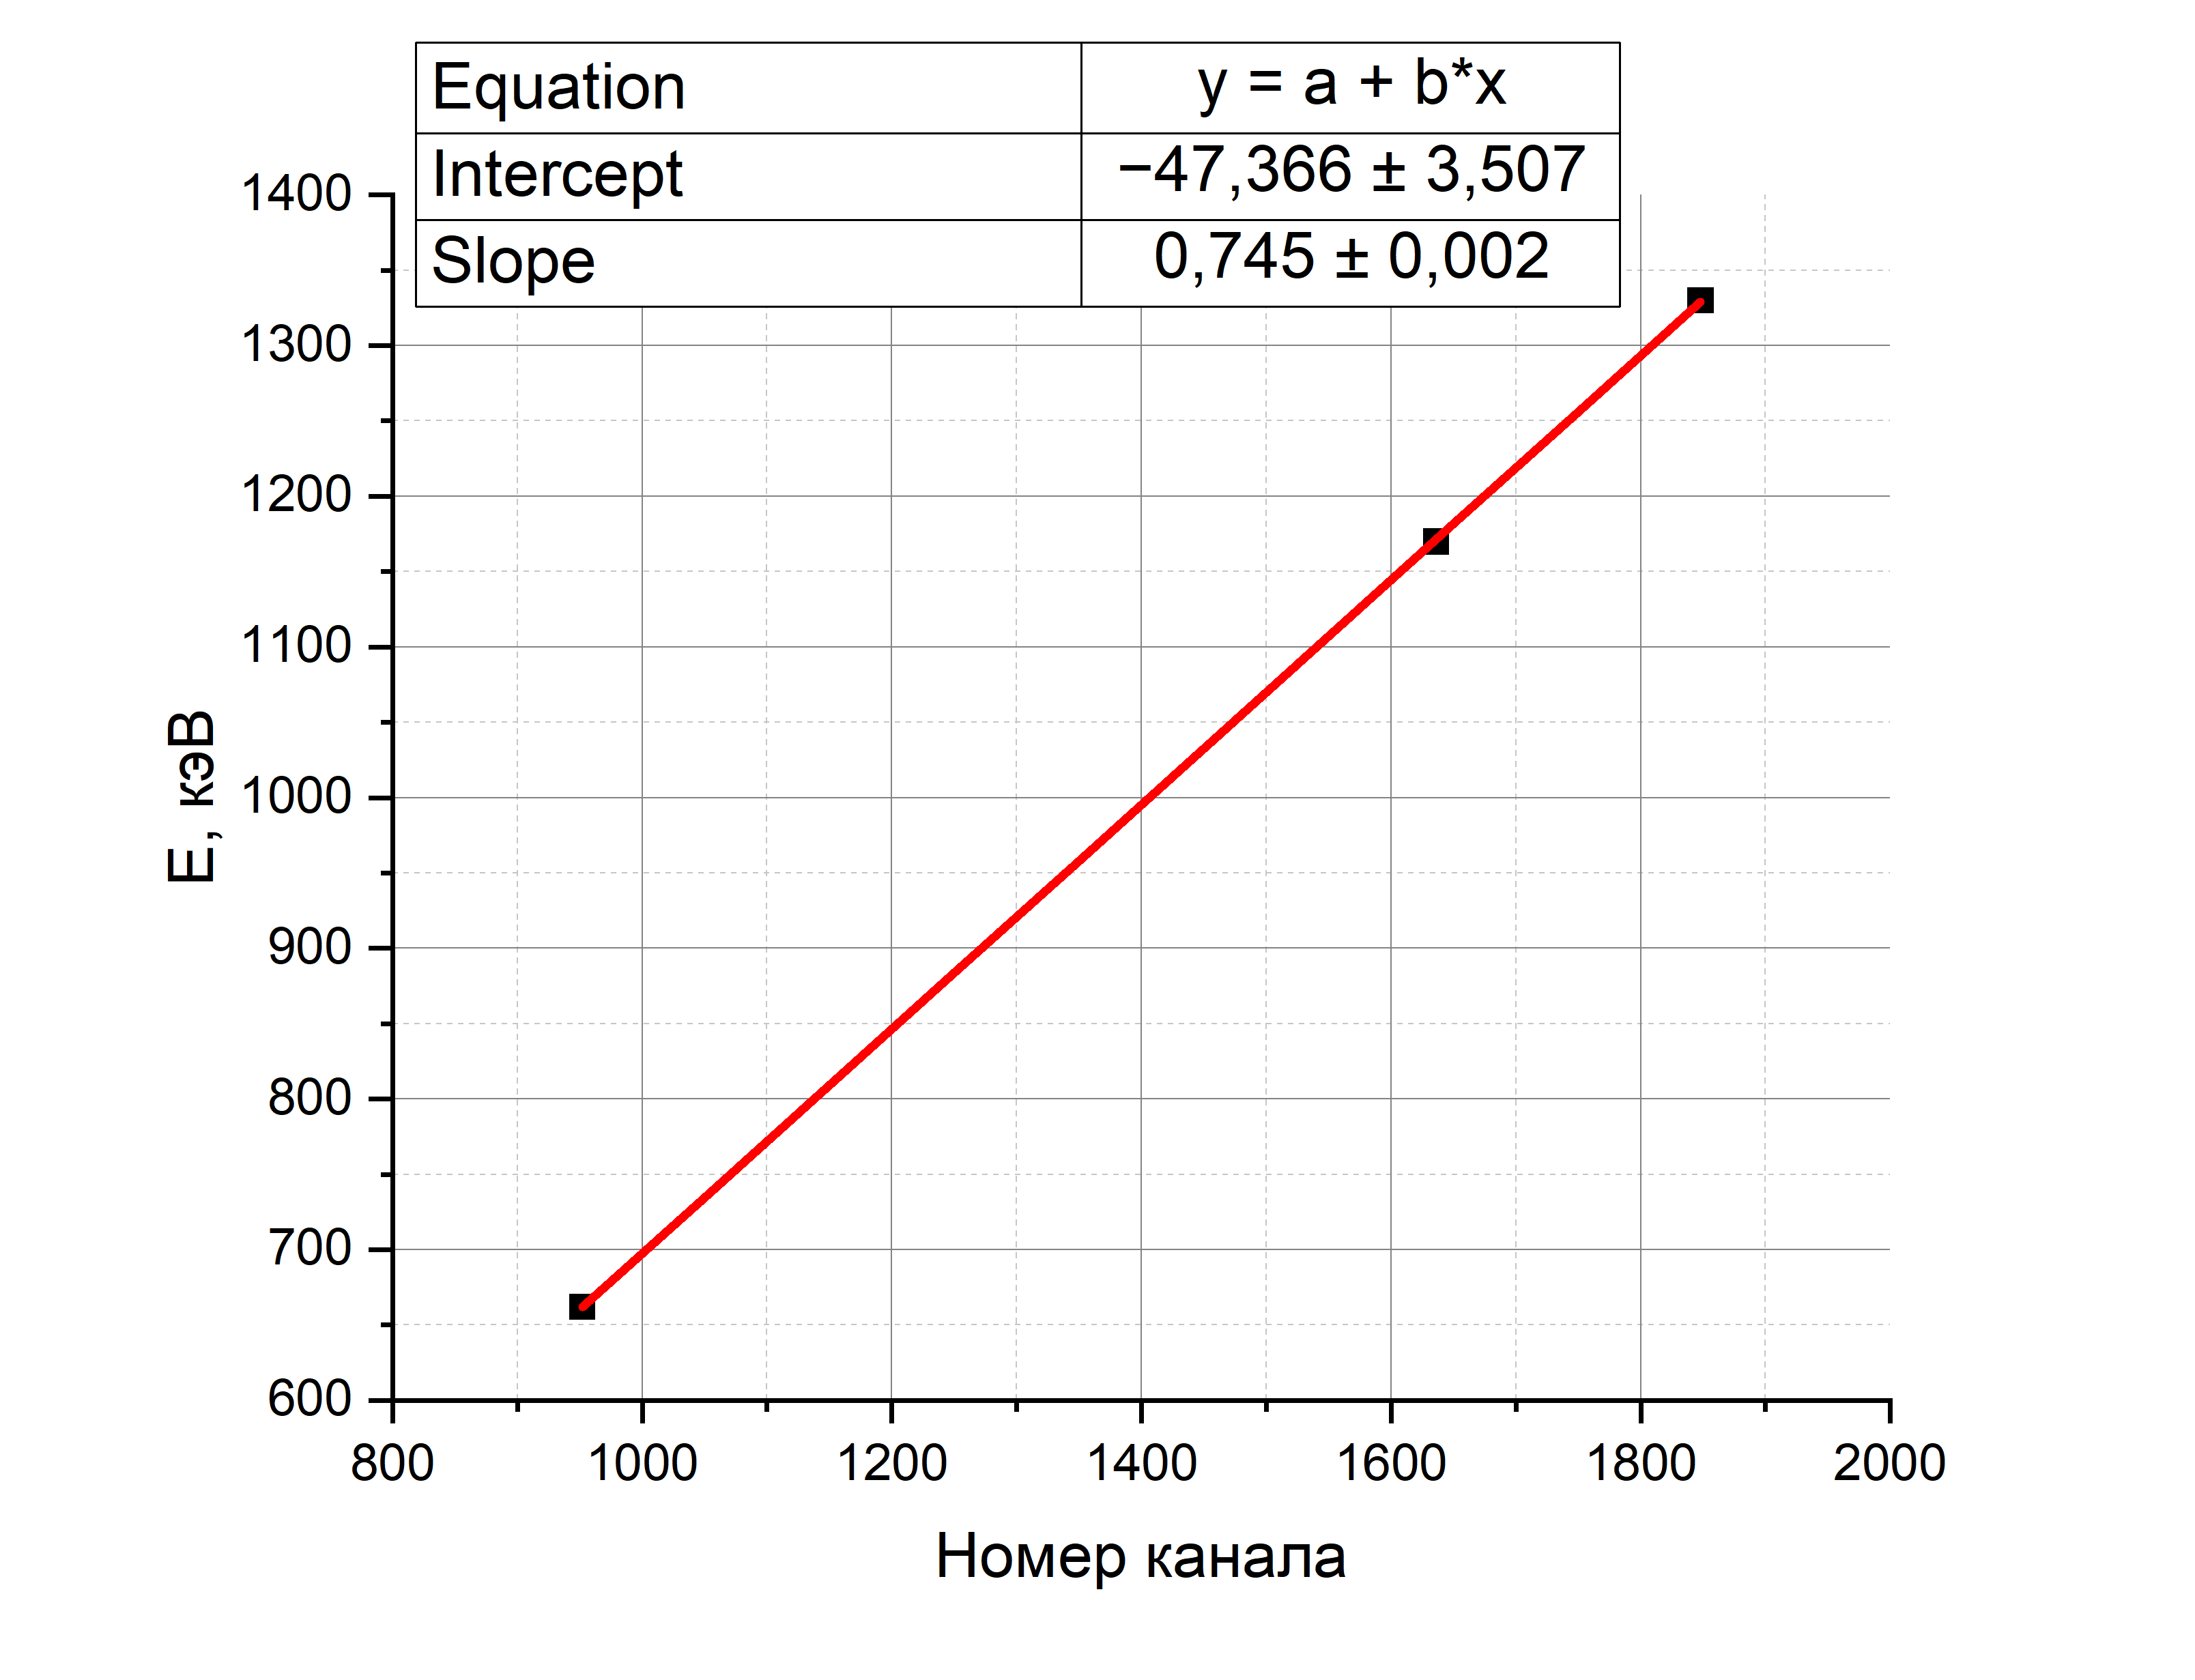
\includegraphics[scale = 0.4]{graph1}
    		\caption{График зависимости $2z_n = f(n)$}
	\end{center}
\end{figure}

\section*{Дифракция Фраунгофера}

Соберем схему согласно рис. 2. 

\begin{figure}[h!]
	\begin{center}
    		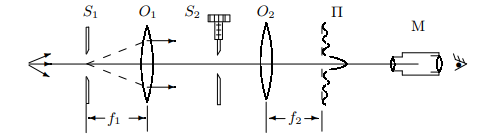
\includegraphics[scale = 1]{fig2}
    		\caption{Схема установки для наблюдения дифракции Фраунгофера на щели}
	\end{center}
\end{figure}

Подберем ширину щели $S_2$ так, чтобы в поле зрения микроскопа появилась дифракционная картина и добьемся наибольшей контрастности картины.

С помощью винта поперечного перемещения микроскопа измерим ширину щели $D = 0,52 \pm 0,02 \ мм$ , а также координаты $X_m$ нескольких дифракционных минимумов. Данные занесем в Таблицу 2.

\begin{table}[h]
\begin{center}
\caption{Зависимость $X_m(m)$}
\begin{tabular}{|c|c|c|c|c|c|c|c|c|c|c|}
\hline
m     & -5  & -4  & -3  & -2  & -1   & 0    & 1    & 2    & 3    & 4   \\ \hline
$X_m$, мм & 1,2 & 1,3 & 1,5 & 1,7 & 1,84 & 1,98 & 2,12 & 2,28 & 2,45 & 2,6 \\ \hline
\end{tabular}
\end{center}
\end{table}

Построим график зависимости $X_m(m)$, учитывая что $\sigma_{X_m} = 0,01 $ мм.

\begin{figure}[h!]
	\begin{center}
    		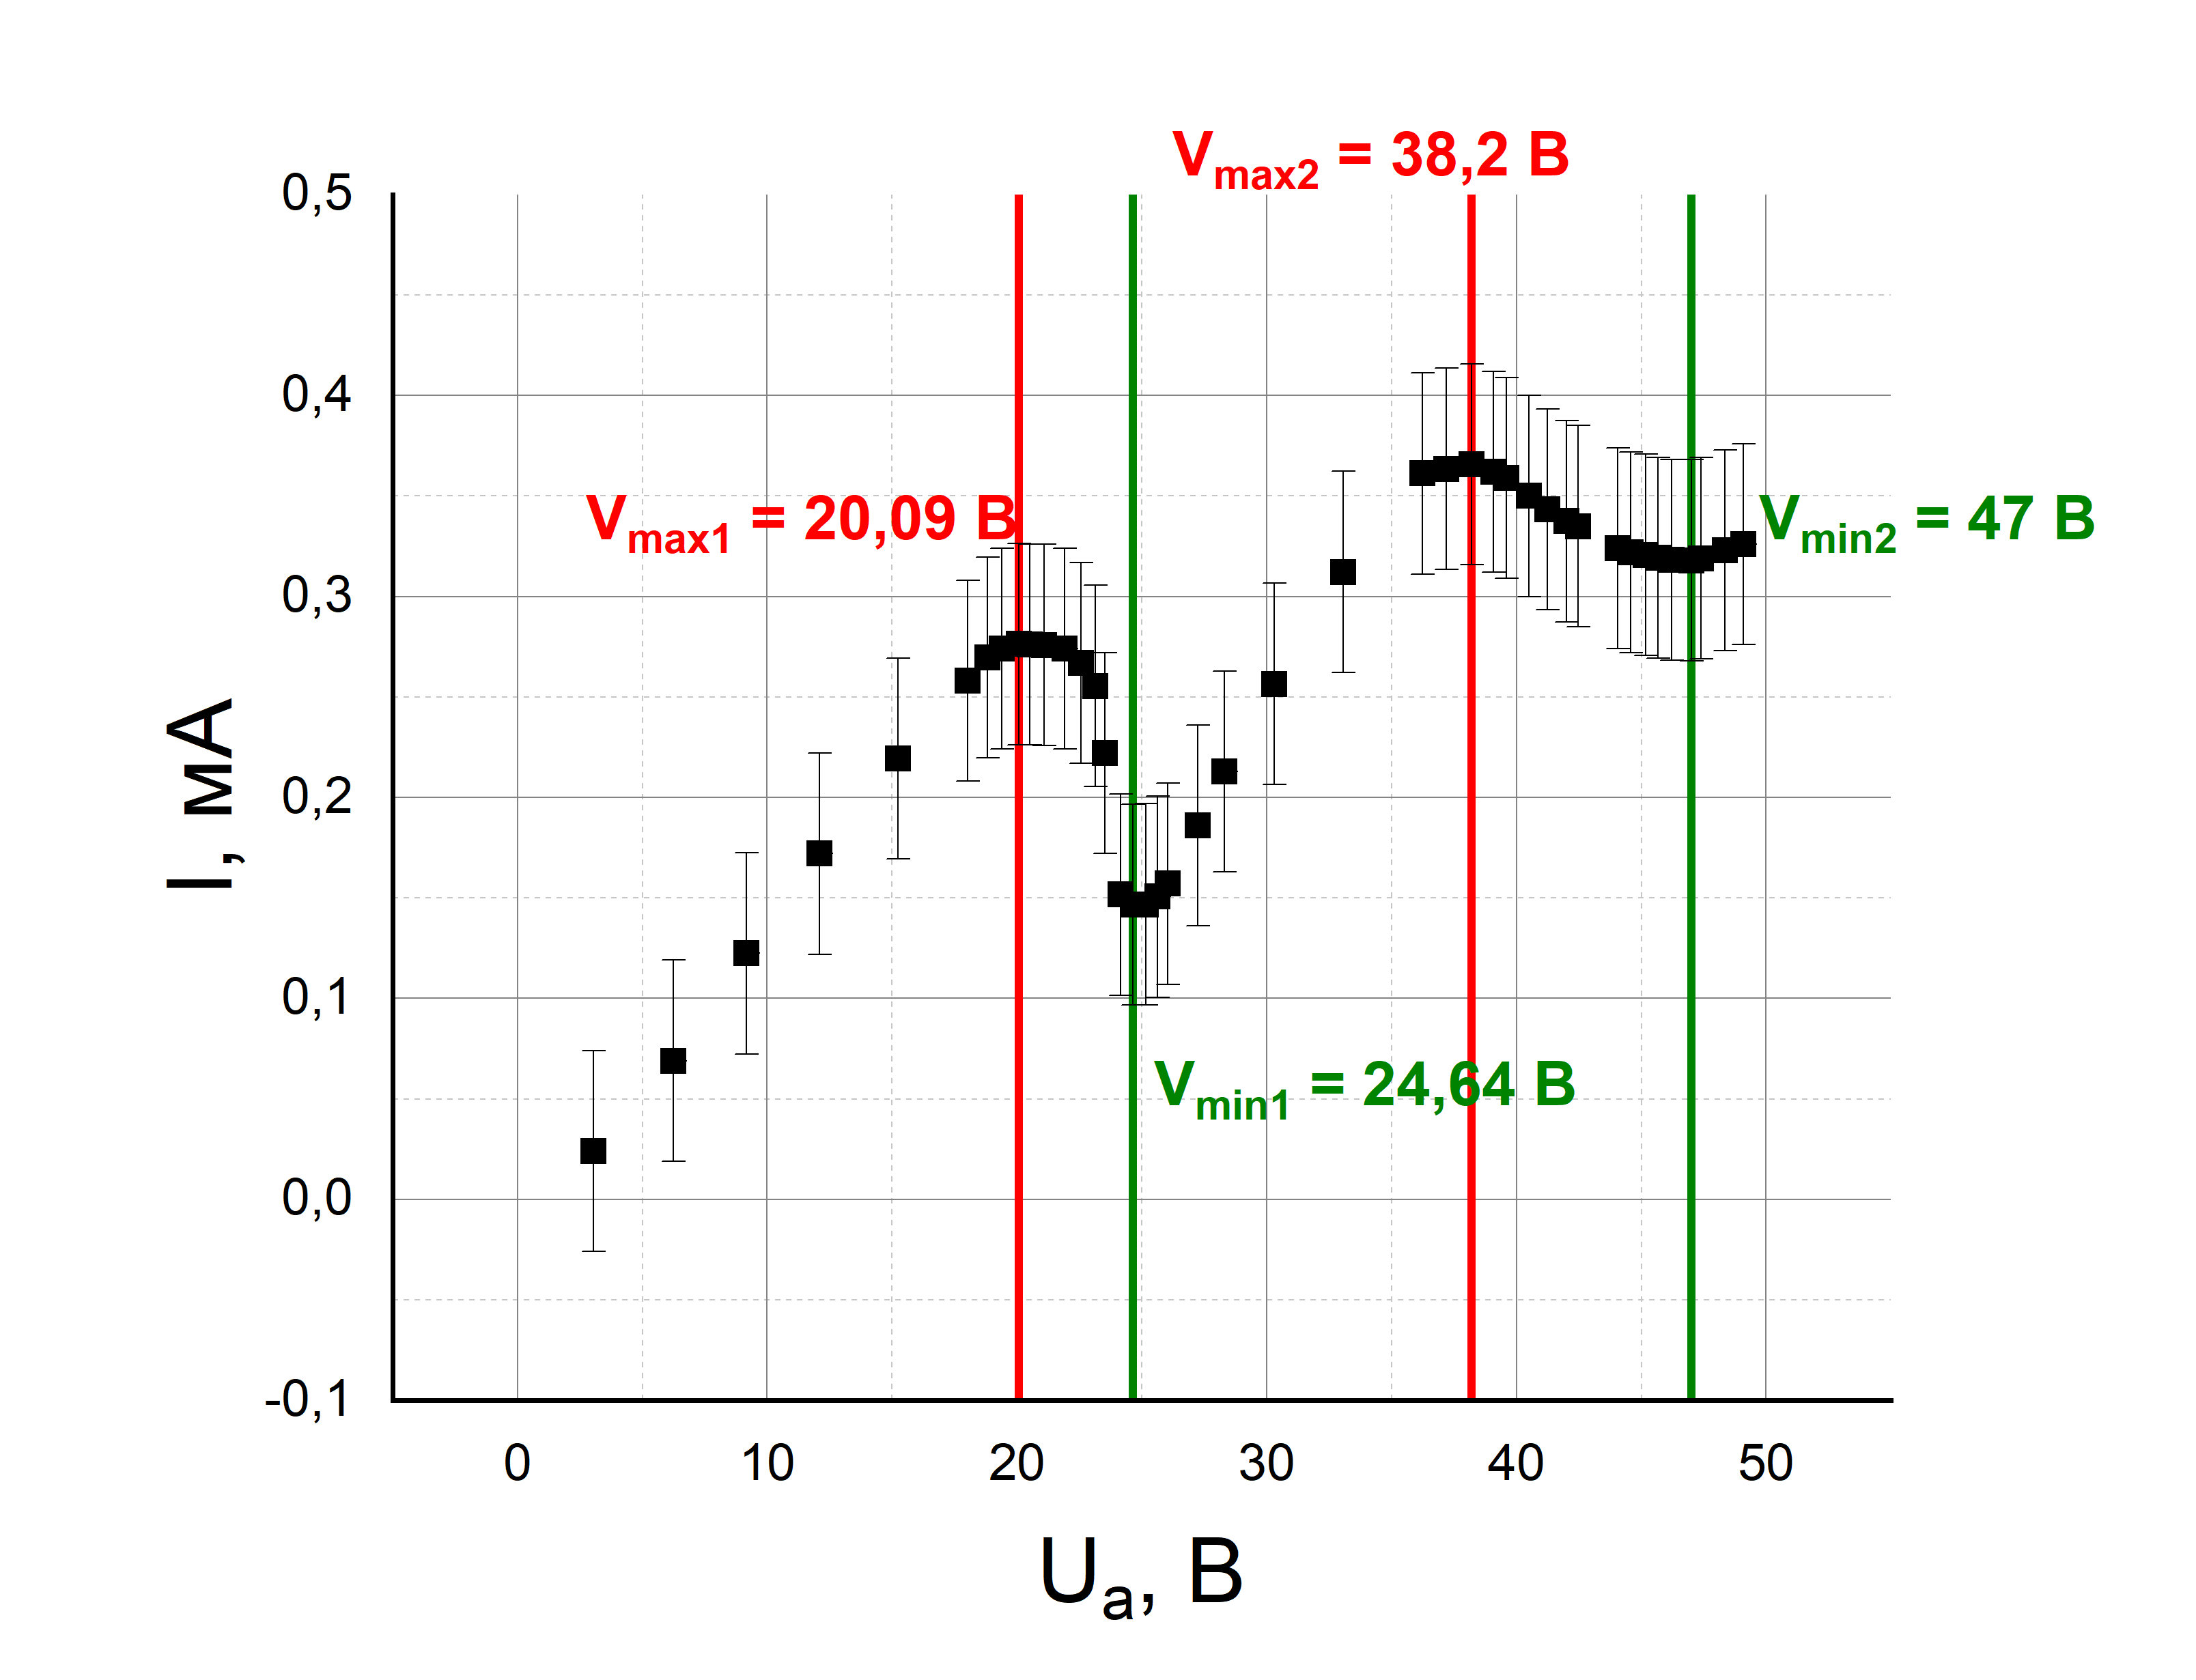
\includegraphics[scale = 0.4]{graph2}
    		\caption{График зависимости $X_m(m)$}
	\end{center}
\end{figure}

Тогда согласно формуле:

$$
X_m = f_2 m \frac{\lambda}{D}
$$

Расстояние между соседними минимумами постоянно и равно наклону графика. 

$$
\Delta X_m = 0,157 \pm 0,003 \ мм
$$

Также рассчитаем ширину щели -- D -- зная фокусное расстояние $f_2 = 11,5 \ см $:

$$
D = f_2 \frac{\lambda}{k} = 0,423 \ мм
$$

$$
\sigma_D = D \frac{\sigma_k}{k} = 0,008 \ мм
$$

Окончательно:

$$
D = 0,423 \pm 0,008 \ мм
$$

\newpage

\section*{Дифракция Фраунгофера на двух щелях}

Соберем схему согласно рис. 3. 

\begin{figure}[h!]
	\begin{center}
    		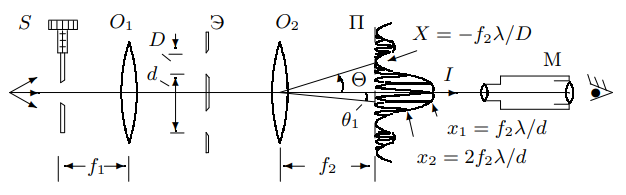
\includegraphics[scale = 1]{fig3}
    		\caption{Схема установки для наблюдения дифракции Фраунгофера на двух щелях}
	\end{center}
\end{figure}

В области главного дифракционного максимума наблюдаем системы равноотстоящих темных и светлых полос. Добьемся четкости дифракционной картины.

С помощью микрометрического винта и поперечных салазок определим: ширину главного максимума -- $h = 0,60 \pm 0,02$мм ; число светлых полос -- n = 18; расстояние между щелями  -- $d = 0,16 \pm 0,2$ мм.

Найдем расстояние между соседними полосами и через него рассчитаем расстояние между щелями:

\begin{gather*}
\delta x = \frac{h}{n} \approx 0,033 \pm 0,001 \ мм \\
%
d = f_2 \frac{\lambda}{\delta x} \approx 0,19 \pm 0,02 \  мм
\end{gather*}

Исследуем влияние пространственной когерентности на видность интерференционной картины. Расширяя входную щель, подберем такую ширину щели $b_0 = 0,285 \pm 0,020 \ мм$, при которой наступает первое исчезновение интерференционных полос.

Сравним ее с расчетом по формуле:

$$
b_0 = f_1 \frac{\lambda}{d} \approx 0,362 \pm 0,012 \ мм
$$

\newpage

\section*{Влияние дифракции на разрешающую способность оптического инструмента}

Соберем схему согласно рис. 4. 

\begin{figure}[h!]
	\begin{center}
    		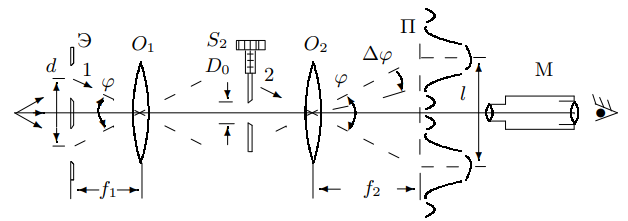
\includegraphics[scale = 1]{fig4}
    		\caption{Схема установки для исследования разрешающей способности оптического инструмента}
	\end{center}
\end{figure}

Подберем ширину щели $S_2$ так, чтобы изобржения обоих щелей почти сливались и запишем показания микрометрического винта (ширину щели) $D_0 = 0,063 \pm 0,02 \ мм$.

Также измерим расстояние между щелями -- $d = 0,16 \pm 0,02 \ мм$, ширина щели -- $b = 0,20 \pm 0,02 \ мм$. Рассчитаем $D_0$ исходя из критерия Релея:

$$
D_0 = \frac{f_1}{d} \lambda \approx 0,043 \\\ мм $$



\section* {Выводы}
В ходе работы было изучено явление дифракции света - дифракция Френеля на щели и на препятствии, дифракция Фраунгофера на одной и двух щелях, а также влияние дифракции на разрешающую способность оптического инструмента

\begin{itemize}
    \item При исследовании явления дифракции Френеля на щели убедились, что ширина зон Френеля примерно равна ширине щели
    
    \item При исследовании явления дифракции Фраунгофера на щели получили значение ширины щели, примерно равно измеренному непосредственно с помощью регулятора ширины щели. Разница обусловлена скорее всего расшатанностью регулятора.
    \begin{center}
        $D_0 = 520 $мкм \hspace{1cm} $D = 423$ мкм
    \end{center}
    
    \item При исследовании явления дифракции Фраунгофера на двух щелях было получено значение расстояния между щелями, примерно равное измеренному с помощью микроскопа:
    
    \begin{center}
        $d_0 = 0,16$ мм \hspace{1cm} $d= 0,19$ мм
    \end{center}
    \item При изучении разрашающей способности, расчет через критерий Релея дал меньший результат, чем подобранный на глаз:
    
    \begin{center}
        $D_0 = 0,063$ мм \hspace{1cm} $D= 0,043$ мм
    \end{center}
\end{itemize}








\end{document}